% f2015zjw_q19_conic.tex — 2015 年高考数学·浙江卷·文科 第 19 题（抛物线与圆）
%
% 【来源】`.work/phase3-b18/source/2015浙江文.pdf`（SHA-256
%   a0e49283fb3d086029ec3c96de7e96cc6118365378ea0a24273c6f58285ec977），
%   第 2 页（合订本页 992）；内容对象 23。逐路径实测见
%   `.work/phase3-b18/figure-inventory.md`。
%
% 【坐标口径】源 PDF 用户空间（原点左下、y 向上）。本图本地坐标
%   (x, y) = (x_page − 571.28, y_page − 576.775)，1 单位 = 1 TeX pt。
%   路径坐标逐点照录内容流（含三次贝塞尔控制点）。
%
% 元素计数：9 条路径（x/y 轴＋箭头、圆、3 直线、抛物线）＋6 个标签
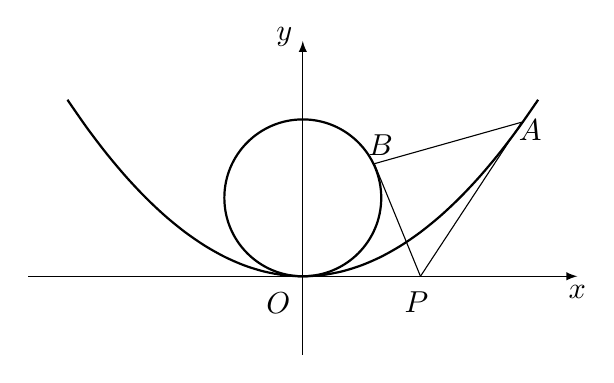
\begin{tikzpicture}[x=1pt, y=1pt,
    every node/.style={inner sep=0pt, font=\fontsize{10.5pt}{12.6pt}\selectfont}]
  \draw[line width=0.3985pt] (0.0002,0.0000)   -- (194.8413,0.0000);
  \fill[line width=0.3985pt] (198.4278,0.0000)   .. controls (197.3651,0.1992) and (195.6383,0.7970) .. (194.4428,1.4944)   -- (194.4428,-1.4944)   .. controls (195.6383,-0.7970) and (197.3651,-0.1993) .. (198.4278,0.0000);
  \draw[line width=0.3985pt] (99.2140,-28.3468)   -- (99.2140,81.4539);
  \fill[line width=0.3985pt] (99.2140,85.0404)   .. controls (99.0148,83.9777) and (98.4170,82.2509) .. (97.7196,81.0554)   -- (100.7084,81.0554)   .. controls (100.0110,82.2509) and (99.4133,83.9777) .. (99.2140,85.0404);
  \draw[line width=0.79701pt] (99.2140,28.3468)   (127.5608,28.3468)   .. controls (127.5608,44.0025) and (114.8697,56.6936) .. (99.2140,56.6936)   .. controls (83.5583,56.6936) and (70.8672,44.0025) .. (70.8672,28.3468)   .. controls (70.8672,12.6911) and (83.5583,0.0000) .. (99.2140,0.0000)   .. controls (114.8697,0.0000) and (127.5608,12.6911) .. (127.5608,28.3468)   -- cycle   (99.2140,28.3468);
  \draw[line width=0.3985pt] (178.3299,55.6871)   -- (125.0495,40.6720);
  \draw[line width=0.3985pt] (141.7342,0.0000)   -- (125.0495,40.6720);
  \draw[line width=0.3985pt] (141.7342,0.0000)   -- (178.3299,55.6871);
  \draw[line width=0.79701pt] (14.1736,63.7803)   .. controls (14.1736,63.7803) and (19.2938,56.2971) .. (21.2603,53.5932)   .. controls (23.2268,50.8892) and (26.3805,46.7500) .. (28.3470,44.2919)   .. controls (30.3135,41.8337) and (33.4672,38.0888) .. (35.4337,35.8764)   .. controls (37.4002,33.6641) and (40.5539,30.3133) .. (42.5204,28.3468)   .. controls (44.4869,26.3803) and (47.6406,23.4237) .. (49.6071,21.7030)   .. controls (51.5736,19.9823) and (54.7273,17.4199) .. (56.6938,15.9451)   .. controls (58.6603,14.4702) and (61.8140,12.3020) .. (63.7805,11.0730)   .. controls (65.7470,9.8439) and (68.9007,8.0699) .. (70.8672,7.0867)   .. controls (72.8337,6.1034) and (75.9874,4.7237) .. (77.9539,3.9863)   .. controls (79.9204,3.2488) and (83.0741,2.2633) .. (85.0406,1.7717)   .. controls (87.0071,1.2800) and (90.1608,0.6887) .. (92.1273,0.4429)   .. controls (94.0938,0.1971) and (97.2475,0.0000) .. (99.2140,0.0000)   .. controls (101.1805,0.0000) and (104.3342,0.1971) .. (106.3007,0.4429)   .. controls (108.2672,0.6887) and (111.4209,1.2800) .. (113.3874,1.7717)   .. controls (115.3539,2.2633) and (118.5076,3.2488) .. (120.4741,3.9863)   .. controls (122.4406,4.7237) and (125.5943,6.1034) .. (127.5608,7.0867)   .. controls (129.5273,8.0699) and (132.6810,9.8439) .. (134.6475,11.0730)   .. controls (136.6140,12.3020) and (139.7677,14.4702) .. (141.7342,15.9451)   .. controls (143.7007,17.4199) and (146.8544,19.9823) .. (148.8209,21.7030)   .. controls (150.7874,23.4237) and (153.9411,26.3803) .. (155.9076,28.3468)   .. controls (157.8741,30.3133) and (161.0278,33.6641) .. (162.9943,35.8764)   .. controls (164.9608,38.0888) and (168.1145,41.8337) .. (170.0810,44.2919)   .. controls (172.0475,46.7500) and (175.2012,50.8892) .. (177.1677,53.5932)   .. controls (179.1342,56.2971) and (184.2544,63.7803) .. (184.2544,63.7803);

  \node[anchor=center] at (92.570,86.415) {$y$};  % 源中心 (663.85,663.19)
  \node[anchor=center] at (181.420,52.865) {$A$};  % 源中心 (752.70,629.64)
  \node[anchor=center] at (127.320,47.215) {$B$};  % 源中心 (698.60,623.99)
  \node[anchor=center] at (90.370,-9.685) {$O$};  % 源中心 (661.65,567.09)
  \node[anchor=center] at (140.320,-9.235) {$P$};  % 源中心 (711.60,567.54)
  \node[anchor=center] at (198.420,-5.585) {$x$};  % 源中心 (769.70,571.19)

\end{tikzpicture}
%
% 【自验结果】
%   探针：latexmk -pdfxe（待跑）。
